

% This is samplepaper.tex, a sample chapter demonstrating the
% LLNCS macro package for Springer Computer Science proceedings;
% Version 2.20 of 2017/10/04
%
\documentclass[runningheads]{llncs}
%
\usepackage[romanian]{babel}
\usepackage{graphicx}
% Used for displaying a sample figure. If possible, figure files should
% be included in EPS format.
%
% If you use the hyperref package, please uncomment the following line
% to display URLs in blue roman font according to Springer's eBook style:
% \renewcommand\UrlFont{\color{blue}\rmfamily}

\begin{document}
%
\title{Poshet}
%
%\titlerunning{Abbreviated paper title}
% If the paper title is too long for the running head, you can set
% an abbreviated paper title here
%
\author{Sabina-Alina Prodan}
%
\authorrunning{S. Prodan}
% First names are abbreviated in the running head.
% If there are more than two authors, 'et al.' is used.
%
\institute{Universitatea "Alexandru Ioan Cuza", Iași, România}
%
\maketitle              % typeset the header of the contribution
%
\begin{abstract}
Poshet este un client pentru serviciul POP3 în care se poate vizualiza, organiza și trimite e-mail. În continuare sunt detaliate atât tehnologiile utilizate, structura aplicației, cât și diverse detalii de implementare.

\renewcommand\keywordname{{\bf Cuvinte cheie:}}

\keywords{Mail \and POP3 \and SMTP \and MIME \and OOP \and wxWidgets}
\end{abstract}
%
%
%
\section{Introducere}

Poshet este un client cu interfață grafică, scris în C++ cu wxWidgets, pentru serviciile de mail electronic POP3 (pentru obținerea de mailuri) și SMTP (pentru trimiterea de mailuri). Printre funcționalitățile acestuia se numără: vizualizarea și organizarea mailurilor primite, trimiterea de mailuri noi cu atașamente, reply sau forwarding la mailuri primite.

\section{Tehnologii aplicate}

Proiectul este scris în C++ utilizând OOP. Pentru compilarea sa sunt folosite atât fișiere \texttt{Makefile}, cât și CMake. Proiectul include un fișier \texttt{README.md} care detaliază procesul de compilare.

Comunicarea în rețea cu serverele POP3 și SMTP se realizează prin intermediul funcțiilor POSIX. Protocolul ales la nivel de transport este TCP, fiindcă ambele protocoale la nivel de aplicație sunt bazate pe acesta.

Comunicarea cu baza de date SQLite creată local se realizează cu ajutorul librăriei SQLite3. În comparație cu alternative precum XML, o bază de date concretă permite interogări mai complexe și o organizare mai ușoară a mailurilor dintr-un inbox.

Pentru interfața grafică este utilizată librăria wxWidgets (în ciuda altor librării precum Qt) datorită simplității sale, a structurii bazate pe OOP și în mod special a integrării sale facile cu Visual Studio Code și CMake.

Pentru analizarea și transformarea mailurilor din format MIME\cite{ref_rfc_mime} într-un format afișabil în client, dar și pentru transpunerea input-ului utilizatorului din fereastra Mail Creator în format MIME, se utilizează o librărie externă, VMime.

Pentru încriptarea SSL, opțională, a conexiunilor POP3 și SMTP se utilizează librăria OpenSSL.


\section{Structura aplicației}


\subsection{Arhitectura principală}

Proiectul folosește clase și OOP, având o structură inspirată de arhitectura MVP (Model-View-Presenter) pentru a separa responsabilitățile între clase.



\subsection{Detalii despre arhitectură}


Principala clasă care face legătura între interfețele aplicației și logica din spate (comunicarea cu servere, cu baza de date, etc.) este AppController. Aceasta administrează și comunică cu instanțe ale interfețelor UsersFrame, LoginFrame, DashboardFrame și MailCreatorFrame, și instanțe ale claselor Session, FileManager, UsersManager și MailBuilder (utilizat când MailCreatorFrame este deschis). Clasa AppController poate fi privită ca un mediator între interfețe și logica programului, delegând operațiuni claselor specializate și trimițându-le interfețelor.

Session este clasa care se ocupă de comunicarea cu resurse externe pentru a obține și furniza informații. Aceasta solicită și trimite informații către instanțe ale altor clase precum FileManager, POP3Connection, SMTPConnection sau DatabaseConnection, care realizează operații precum: crearea unui mailbox (sau potrivirea cu un mailbox deja existent) pentru utilizatorul conectat, obținerea mailurilor noi, salvarea lor în baza de date locală și în fișierele corespunzătoare, trimiterea unui mail nou, sau salvarea locală a unui atașament dintr-un mail.

În momentul primirii de notificări de la interfețele la care AppController este "abonat", AppController se ocupă de interacțiunea cu clasa Session pentru a obține informații și a le transmite către interfețe, care trebuie să folosească datele pentru a se actualiza și a le afișa către utilizator.

Datele care aparțin unui mail sunt păstrate la runtime cu ajutorul clasei Mail, care conține metode prin care se poate procesa conținutul unui buffer ASCII (scris conform standardului MIME) și se pot obține informații precum headers, conținutul plain-text sau HTML, atașamente, etc. În momentul când se dorește afișarea conținutului mailului pe ecran, interfața DashboardFrame este responsabilă cu afișarea datelor mailului în viewMailPanel, utilizând elemente specializate ale wxWidgets precum wxTextCtrl pentru plain-text sau wxHTMLWindow pentru conținut HTML cu imagini inline.


\subsection{Stocarea informațiilor}

La momentul deschiderii programului, în același folder cu executabilul se crează folderul \texttt{.poshet}, unde sunt create folderul \texttt{mail} (unde sunt stocate conținuturile "raw" ale mailurilor, în fișiere individuale) și baza de date SQLite \texttt{mail.db} cu tabelele \texttt{mail} în care sunt stocate informații despre utilizatorul căruia îi aparține un mail, filename-ul unde poate fi găsit în folderul amintit mai sus, sau tag-ul care i-a fost asignat de către utilizator mailului respectiv, și \texttt{users} cu informațiile și setările utilizatorilor.


\begin{figure}
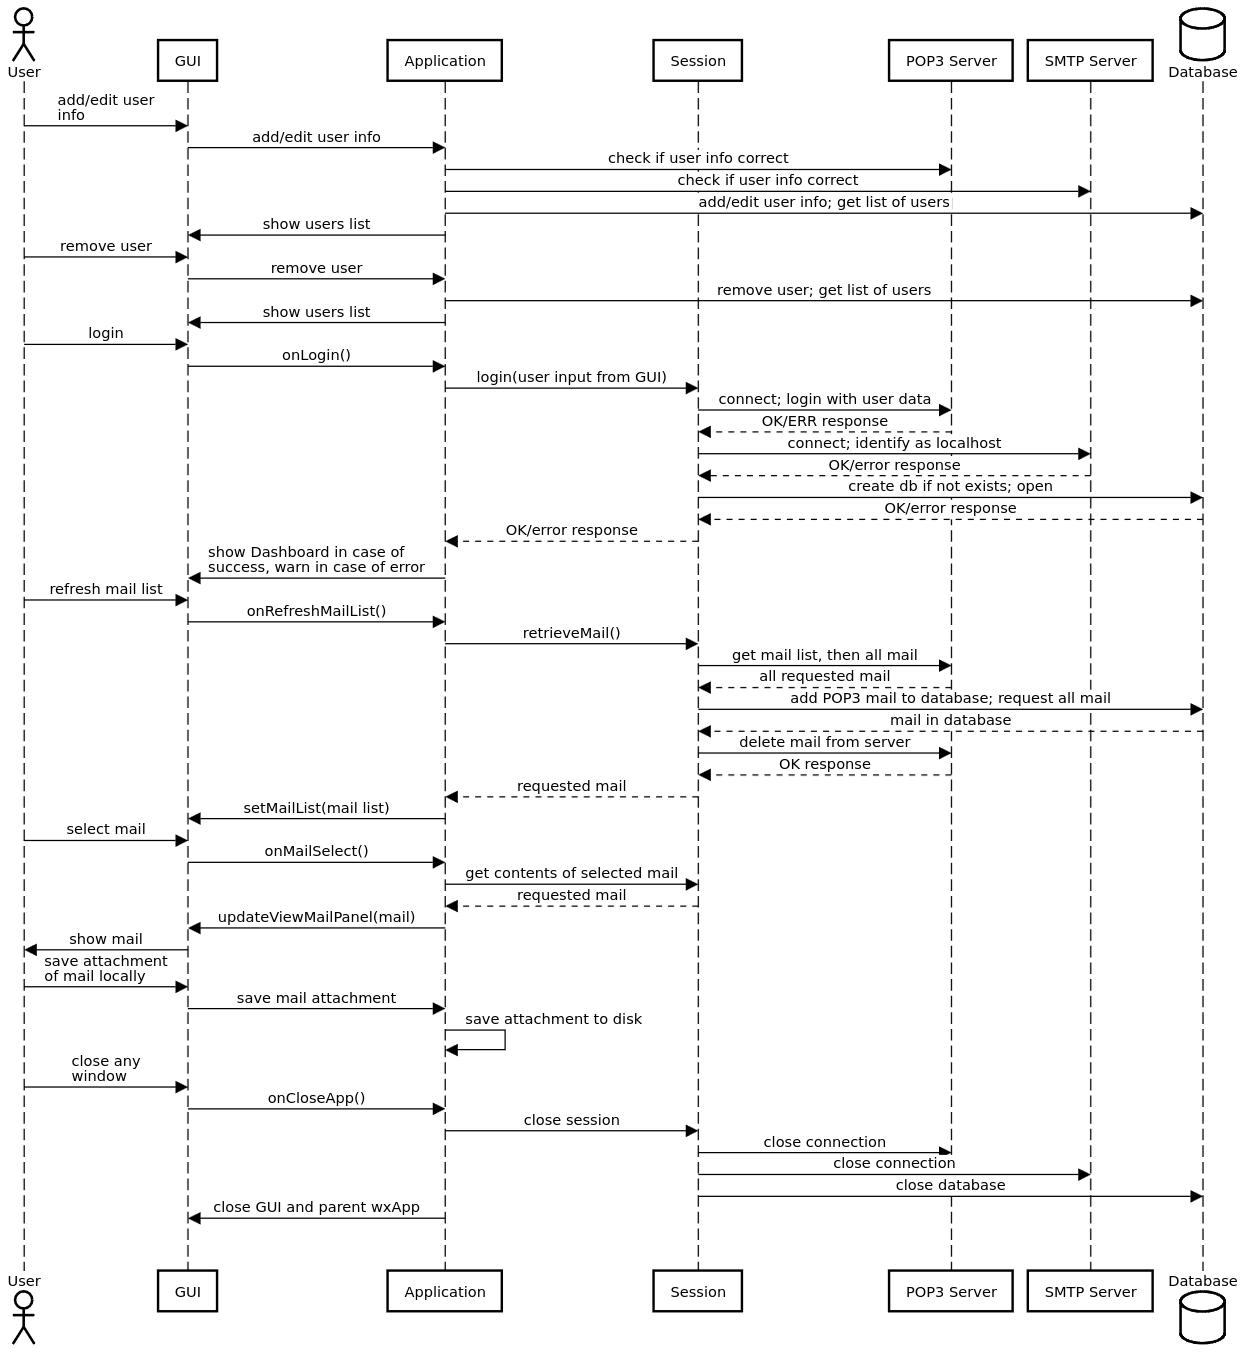
\includegraphics[width=\textwidth]{POSHET1.png}
\caption{Diagrama secvențială a aplicației, partea 1: aici sunt ilustrate mecanismele de logare, afișare a mailurilor primite, și închidere a aplicației.} \label{firsthalf}
\end{figure}

\begin{figure}
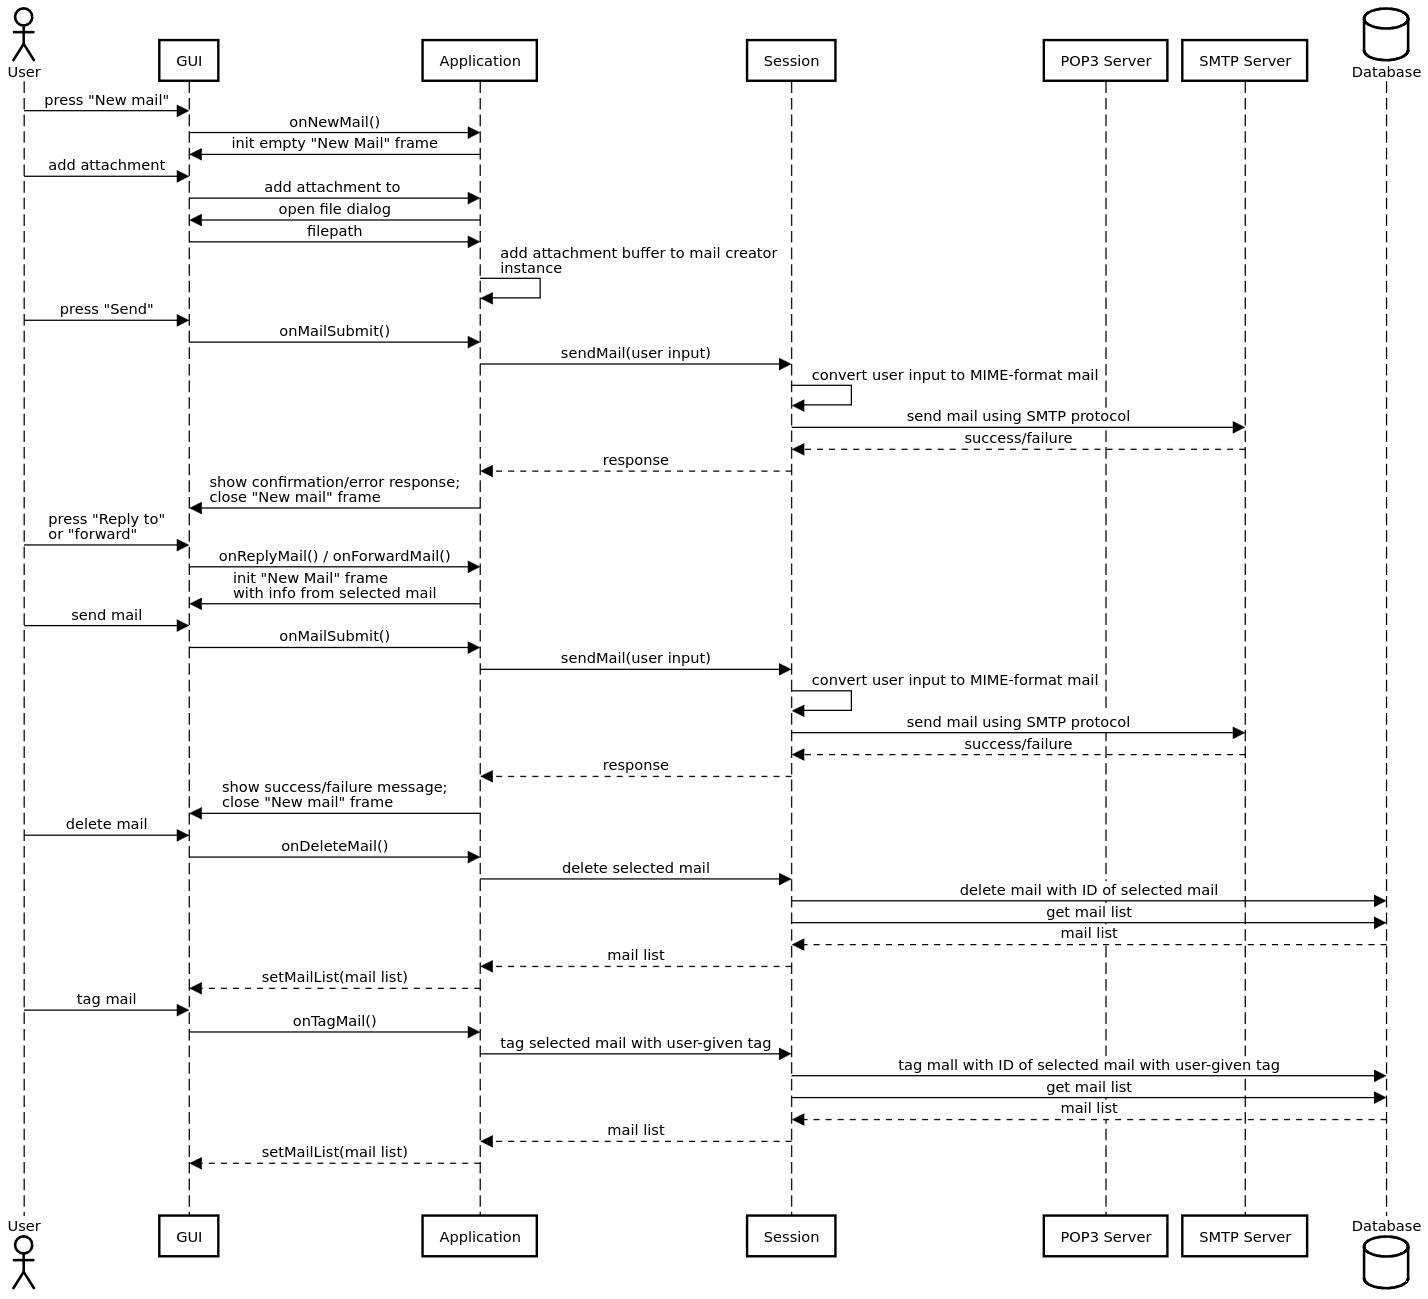
\includegraphics[width=\textwidth]{POSHET2.png}
\caption{Diagrama secvențială a aplicației, partea 2: aici sunt ilustrate mecanismele de trimitere de mail nou și organizare de mail primit.} \label{secondhalf}
\end{figure}


\newpage




\section{Aspecte de implementare}

\subsection{Protocoale utilizate}
Proiectul constă într-un client pentru servere existente, deci acesta se folosește de protocoale la nivel de aplicație deja existente.

Pentru obținerea mailurilor se folosește protocolul POP3\cite{ref_rfc_pop3}, iar pentru trimiterea de mailuri se folosește protocolul SMTP\cite{ref_rfc_smtp}. Clasele responsabile de conexiunile POP3 și SMTP trimit comenzi corespunzătoare funcționalităților dorite de utilizator, recunoscute de servere; spre exemplu, \texttt{USER} / \texttt{PASS} pentru autentificare POP3, \texttt{RETR} pentru lista de mailuri, \texttt{LIST} pentru datele unui mail particular, \texttt{MAIL TO} și altele pentru trimiterea unui mail, etc.

Ambele protocoale sunt de tip comandă-răspuns; așadar, în urma trimiterii comenzii se așteaptă răspuns afirmativ (sau un mesaj de eroare) de la server, informația fiind apoi transmisă la funcțiile care au solicitat-o.

\subsection{Scenarii de utilizare}
Poshet este menit să comunice cu un server POP3 (printr-o conexiune ori ne-încriptată, ori încriptată prin SSL, cu autentificare plain-text prin comenzile \texttt{USER} și \texttt{PASS}), și cu un server SMTP (cu SSL sau nu, cu autentificare de tip \texttt{AUTH LOGIN} sau fără autentificare). Proiectul a fost testat atât cu adrese \texttt{@localhost} (cu un server Dovecot atât cu SSL, cât și fără, și un server Postfix, fără SSL, fără autentificare), dar și cu o adresă personală Yahoo (cu serverele \texttt{pop.mail.yahoo.com:995} și \texttt{smtp.mail.yahoo.com:465}, cu autentificare SMTP de tip \texttt{AUTH LOGIN}).

Un client de acest tip poate fi utilizat pentru a citi mail atât de pe adrese locale, pe \texttt{localhost}, dar și de pe adrese de la furnizori care permit modalitățile de conectare și autentificare amintite mai sus.

Când se adaugă un mailbox nou (sau se editează unul existent) este suficient să se introducă o adresă de email și o parolă, în urma cărora aplicația va încerca să intuiască parametri precum domain name-ul serverelor POP3 și SMTP, sau username-ul pentru mailbox-ul POP3. Dacă autentificarea sau conectarea eșuează, există și posibilitatea de a le introduce manual, prin field-urile marcate cu "(Optional)". Informațiile sunt verificate pe rețea și apoi salvate local, în baza de date, iar utilizatorul poate ulterior alege mailbox-ul pe care dorește să îl acceseze.

După logare va fi afișată fereastra de tip "dashboard", care va afișa lista curentă de mailuri. Dacă este selectat vreunul, se afișează conținutul și detaliile acestuia în partea dreaptă a ecranului, precum și atașamentele sale. În partea stângă a ferestrei se regăsesc și alte elemente, precum butoane de trimitere de mail nou, reîmprospătare, sau vizualizarea mailurilor cu un anumit tag.

În fereastra de creare de mail-uri se poate introduce doar plaintext (de altfel, și reply-urile/forward-urile sunt inițializate folosind doar plaintext-ul mail-urilor la care se face referință). Se pot adăuga și șterge, de asemenea, și atașamente. În final, când se trimite un mail, se deschide o conexiune SMTP, se trimite mail-ul, după care conexiunea SMTP este închisă, iar conexiunea POP3 reîmprospătată.

\begin{figure}
    \centering
    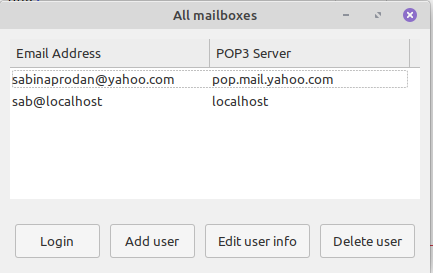
\includegraphics[width={300px}]{allMailboxes.png}
    \caption{Fereastra "All mailboxes".}
    \label{fig:allMailboxes}
\end{figure}

\begin{figure}
    \centering
    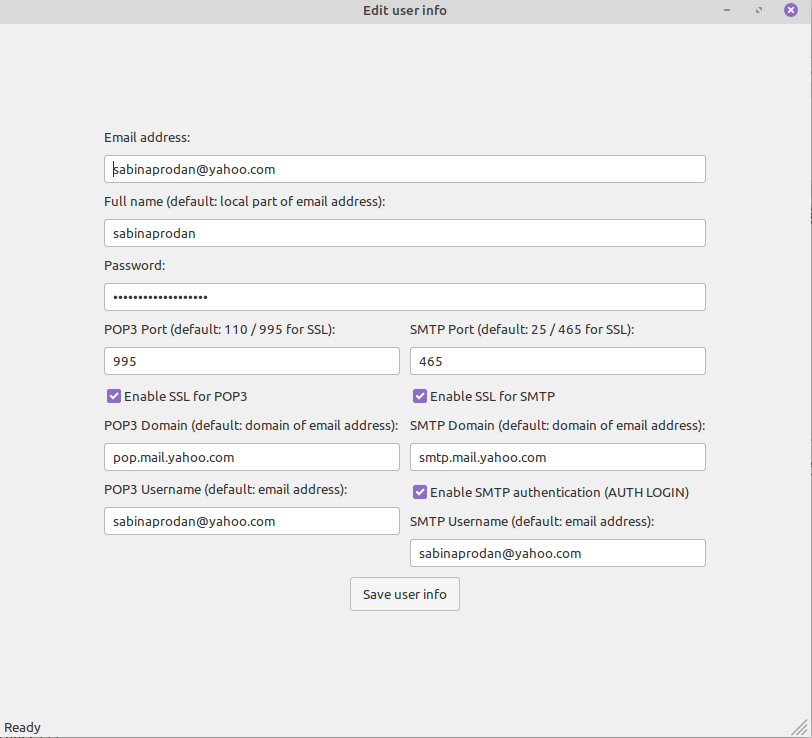
\includegraphics[width={300px}]{editUserInfo.png}
    \caption{Fereastra "Edit user info".}
    \label{fig:editUserInfo}
\end{figure}

\begin{figure}
    \centering
    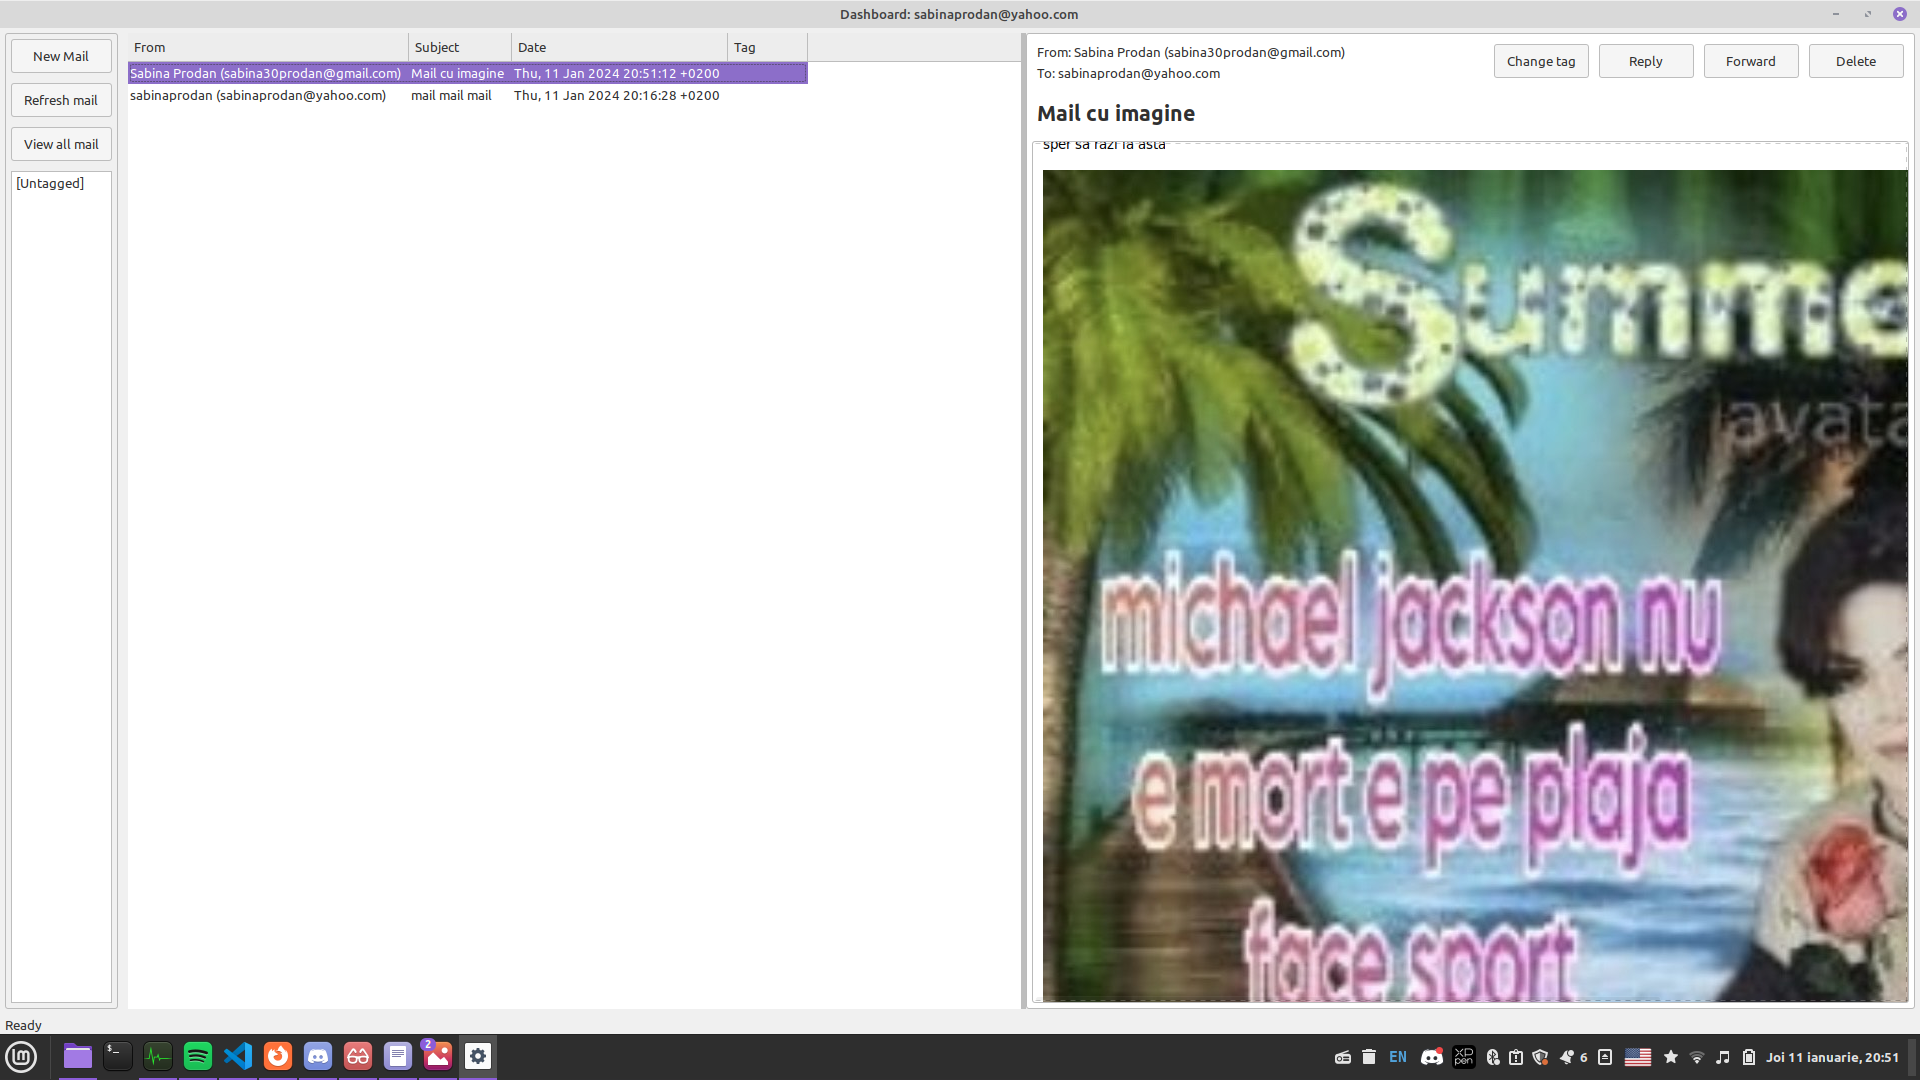
\includegraphics[width=\textwidth]{dashboard.png}
    \caption{Fereastra "Dashboard".}
    \label{fig:dashboard}
\end{figure}

\begin{figure}
    \centering
    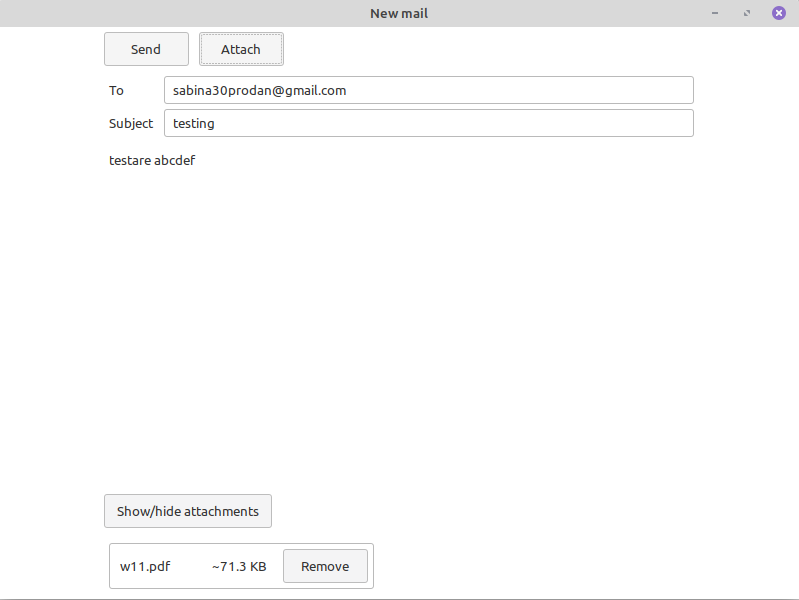
\includegraphics[width=\textwidth]{newMail.png}
    \caption{Fereastra de tip "New mail".}
    \label{fig:newmail}
\end{figure}

\newpage

\subsection{Aspecte interesante legate de implementare}

\subsubsection*{"ConnectionBase".} Atât conexiunea POP3, cât și cea SMTP, folosesc socket-uri TCP, cu sau fără încriptare SSL. Pentru a face implementarea acestora mai ușoară a fost creată clasa de bază \texttt{ConnectionBase}, care reprezintă un wrapper peste un socket, cu propriile metode I/O în funcție de anumite setări. Clasele \texttt{SMTPConnection} și \texttt{POP3Connection} sunt derivate ale acestei clase.

\subsubsection{Administrarea conexiunilor POP3 și SMTP.}

Conexiunile cu serverele POP3 și SMTP sunt administrate de clasele POP3Connection și SMTPConnection, care asigură comunicarea corectă cu acestea conform protocoalelor corespunzătoare. 

În general, după o anumită perioadă de inactivitate configurată de către administratorii serverelor, acestea pot încheia conexiunea. Acest fapt nu este o problemă pentru SMTPConnection, fiindcă o conexiune SMTP nu trebuie să fie persistentă. În program, o conexiune SMTP este deschisă doar la logare (pentru a verifica corectitudinea datelor de logare) și în momentul în care este necesară trimiterea unui mail, fiind închisă imediat după. În schimb, conexiunea POP3 a fost proiectată în așa fel încât să poată fi persistentă, acomodând pentru un timp mai lung de procesare a unui mail după obținerea sa de la server. O particularitate interesantă a clasei POP3Connection este folosirea unui \texttt{std::thread} pentru a menține conexiunea activă: acesta trimite la un anumit interval repetat de timp, conform protocolului POP3, o operație de tip "no-op", prin care să semnaleze activitate fără a realiza o operație propriu-zisă.

În POP3Connection există membrul \texttt{std::thread \_noopThread}, și o metodă \texttt{keepAlive()} care este executată de către acest thread. Pentru ca "no-op"-urile trimise de acest thread să nu interfereze cu procesul comandă-răspuns se folosește un \texttt{\_commandMutex}, folosit în funcția \texttt{execCommand} care este apelată atât de comenzi reale, cât și de comanda "no-op". De asemenea, mutexul \texttt{\_stateMutex} este utilizat, printre altele, pentru a actualiza și verifica în mod sigur statusul curent al conexiunii.

Dacă apare o eroare (închiderea remote a conexiunii, sau timeout) în timp ce se dorește trimiterea unui "no-op", thread-ul își încheie execuția. Thread-ul principal va reverifica existența unei conexiuni active când va încerca să comunice la rândul ei cu serverul POP3, și va încerca reconexiunea.


\subsubsection{Notificarea între clase.} AppController este notificat când au loc modificări atât la nivel de interfață, cât și la nivel de "business-logic".

Pentru a putea informa legat de input-ul utilizatorului, clasele de interfață grafică își definesc propriile ID-uri pentru \texttt{wxEvent}-uri personalizate pentru diversele abilități ale programului. AppController se "abonează" apoi la interfețele grafice, ascultând pentru diversele evenimente, prin funcția \texttt{Bind()} specifică wxWidgets. În cazul claselor de tip business-logic, care ar trebui să fie cât mai separate de interfața grafică, AppController implementează unele interfețe (clase pur virtuale) și se poate abona la instanțele Session sau MailBuilder pe care le administrează.


\begin{figure}
    \centering
    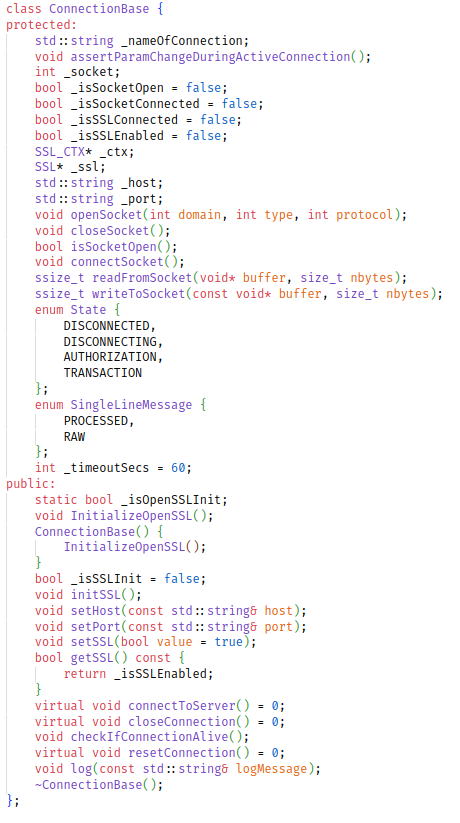
\includegraphics[width=\textwidth]{connectionBase.png}
    \caption{Declararea clasei \texttt{ConnectionBase}.}
    \label{fig:connectionBase}
\end{figure}

\begin{figure}
    \centering
    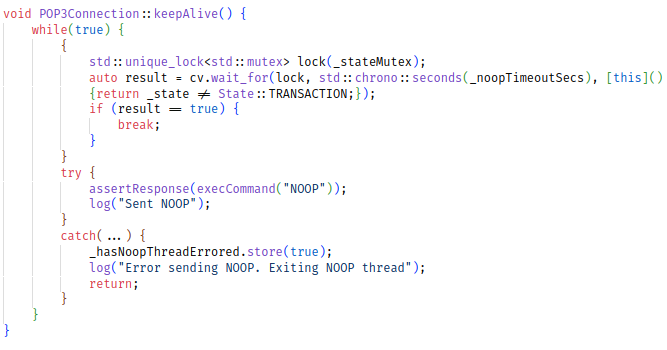
\includegraphics[width=\textwidth]{keepAlive.png}
    \caption{Definiția \texttt{keepAlive()} în \texttt{POP3Connection.cpp}.}
    \label{fig:keepalive}
\end{figure}

\begin{figure}
    \centering
    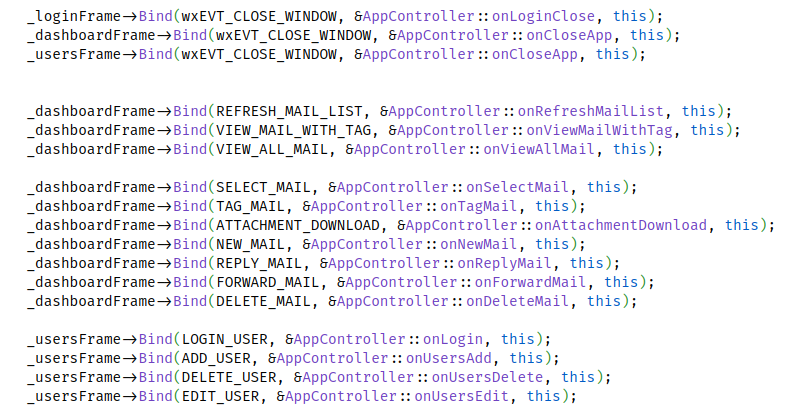
\includegraphics[width=\textwidth]{binding.png}
    \caption{Legarea \texttt{AppController} de principalele interfețe grafice ale programului.}
    \label{fig:wxEvents}
\end{figure}

\begin{figure}
    \centering
    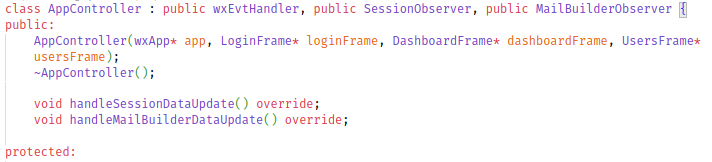
\includegraphics[width=\textwidth]{appControllerSubscribe.png}
    \caption{Parte din definiția \texttt{AppController}, care implementează interfețe pur virtuale de tip "Observer", putându-se astfel "abona" la \texttt{Session} sau \texttt{MailBuilder}.}
    \label{fig:subscribers}
\end{figure}

\newpage

\section{Concluzii}

Clientul Poshet este în principal single-threaded, folosind mai multe fire de execuție doar pentru a menține activă conexiunea POP3. O îmbunătățire posibilă ar fi adăugarea mai multor fire de execuție și modularizarea codului pentru a permite încărcarea mailurilor din inboxul POP3 "in the background" (pentru ca interfața să nu apară ca fiind "not responding" în timpul acestui proces), dar și pentru a putea întrerupe procesul dacă se dorește acest lucru.

Clientul șterge toate mailurile POP3 de pe server imediat după salvarea lor locală. O îmbunătățire ar putea fi adăugarea unei setări care să permită ștergerea mai târzie a mailurilor de pe server, spre exemplu la o zi sau o săptămână după ce au fost salvate.

Clientul poate vizualiza mailuri cu imagini inline, dar nu le poate și trimite. O îmbunătățire la trimiterea de mail nou ar putea fi posibilitatea de adăugare de imagini inline în mail, similar cu alți clienți de mail cunoscuți.

De asemenea, librăria wxWidgets are propriile limitări. Comparativ cu alte librării precum Qt, widget-ul \texttt{wxRichTextCtrl} nu permite importarea fișierelor HTML, ceea ce limitează anumite abilități precum "Reply" și "Forward" la a funcționa în format plaintext. O îmbunătățire ar putea fi portarea proiectului la o altă librărie grafică cu un editor HTML de tip WYSIWYG ("what you see is what you get") precum Qt, sau dezvoltarea unui propriu "handler" bazat pe wxWidgets care să permită importarea HTML.
%
% ---- Bibliography ----
%
% BibTeX users should specify bibliography style 'splncs04'.
% References will then be sorted and formatted in the correct style.
%
% \bibliographystyle{splncs04}
% \bibliography{mybibliography}

\begin{thebibliography}{8}
\bibitem{ref_rfc_pop3}
RFC 1939, \url{https://www.ietf.org/rfc/rfc1939.txt}. Accesat cel mai recent pe 14 Dec 2023

\bibitem{ref_rfc_smtp}
RFC 5321, \url{https://www.ietf.org/rfc/rfc5321.txt}. Accesat cel mai recent pe 14 Dec 2023

\bibitem{ref_rfc_mime}
RFC 2045, \url{https://datatracker.ietf.org/doc/html/rfc2045}. Accesat cel mai recent pe 14 Dec 2023

\bibitem{ref_wxwidgets}
Pagina principală wxWidgets, \url{https://www.wxwidgets.org/}. Accesat cel mai recent pe 14 Dec 2023


\end{thebibliography}
\end{document}
